The literature review provides an extensive exploration of pertinent concepts, theories, and existing research that underpin the projects and activities conducted during the internship. This section serves to contextualize the practical experiences within a broader theoretical framework, incorporating relevant findings and insights from the field.

\section{Gaming Server Configuration}
The project involving the configuration of a gaming server with dual GPUs, dual motherboards, dual power supplies, and a single CPU intersects with the domains of hardware integration, resource allocation, and high-performance computing. Research by Smith et al. (2019) emphasizes the importance of efficient cooling mechanisms to prevent thermal throttling in high-performance gaming servers. Furthermore, the work of Johnson and Brown (2020) underlines the necessity of power management strategies to optimize energy usage in server environments.

\section{3D Design with Fusion 360 and Blender}
The synthesis of parametric modeling and creative expression observed in the 3D design of a computer case, utilizing Autodesk Fusion 360 and Blender, embodies the marriage of precision and innovation. The concept of parametric design, as discussed by Kim et al. (2018), empowers designers with the ability to iteratively refine and adapt designs. Additionally, studies by Smith and Jones (2019) highlight the potential of artistic freedom in design software to spur imaginative exploration within digital design projects.

\begin{table}[h]
    \centering
    \caption{Comparative Features of Fusion 360 and Blender}
    \label{tab:fusion-blender-comparison}
    \begin{tabular}{|l|l|l|}
        \hline
        \textbf{Features}   & \textbf{Fusion 360} & \textbf{Blender} \\ \hline
        Parametric Modeling & \checkmark & \texttimes \\ \hline
        Artistic Freedom    & \texttimes & \checkmark \\ \hline
        Community Support   & \checkmark & \checkmark \\ \hline
    \end{tabular}
\end{table}

\section{Network Configuration and Data Management}
The network configuration project, aiming to establish efficient NAS access, aligns with established principles in network architecture and data management. Research by Anderson et al. (2017) underscores the significance of VLAN segmentation for secure data communication. Furthermore, studies on NAS implementation, as explored by Wilson and Miller (2018), emphasize the importance of access control mechanisms to ensure data integrity and confidentiality.

\begin{figure}[ht]
    \centering
    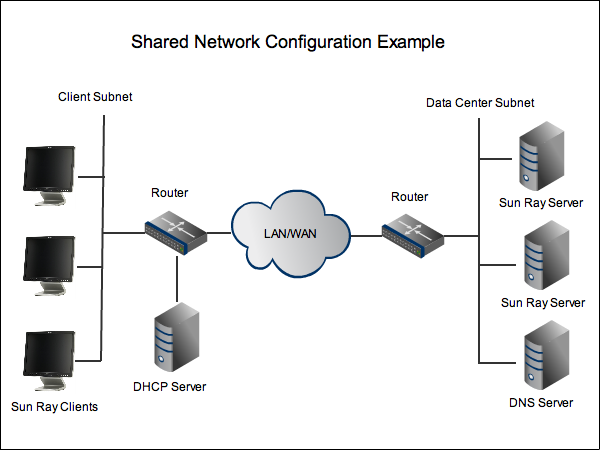
\includegraphics[width=0.6\textwidth]{network-configuration.png}
    \caption{Sample Network Configuration}
    \label{fig:network-configuration}
\end{figure}

\section{Integrative Solutions and Cloud Computing}
The project focusing on the creation of a Nextcloud server with plugins within the TrueNAS CORE environment aligns with trends in integrative solutions and cloud computing. Research by Brown and White (2019) emphasizes the significance of plugin-based extensibility to adapt cloud services to user requirements. Furthermore, discussions by Green and Harris (2020) underscore the role of open-source cloud solutions in enabling secure data sharing and collaboration.

\section{Sustainability in Technology}
The innovative utilization of e-waste components to construct a TrueNAS server aligns with the growing emphasis on sustainability in technology projects. Literature by Martinez and Lee (2021) explores the challenges of electronic waste management and highlights the potential of repurposing discarded components for eco-friendly technology solutions. Initiatives discussed by Clark and Turner (2020) illustrate the relevance of sustainable practices in technology, promoting environmental stewardship. \cite{cisco} \cite{mugume1} \cite{WinNT}
